\section{Introduction}
\label{sec:intro}

Self-supervised learning on a general-domain text corpus followed by end-task learning is the two-staged training approach that enabled deep-and-wide Transformer-based networks \citep{transformer} to advance language understanding \citep{bert, xlnet, ernie, roberta}. However, state-of-the-art models have hundreds of millions of parameters, incurring a high computational cost. Our goal is to realize their gains under a restricted memory and latency budget. We seek a training method that is \emph{well-performing}, \emph{general} and \emph{simple} and can leverage additional resources such as unlabeled task data.

Before considering compression techniques, we start with the following research question: \emph{Could we directly train small models using the same two-staged approach?} In other words, we explore the idea of applying language model (LM) pre-training and task fine-tuning to compact architectures directly. This simple baseline has so far been overlooked by the NLP community, potentially based on an underlying assumption that the limited capacity of compact models is capitalized better when focusing on the end task rather than a general language model objective. Concurrent work to ours proposes variations of the standard \ptft procedure, but with limited generality \citep{patient_kd, distil_bert}. We make the surprising finding that \ptft in its original formulation is a competitive method for building compact models.

For further gains, we additionally leverage knowledge distillation \citep{distillation}, the standard technique for model compression. A compact student is trained to recover the predictions of a highly accurate teacher. In addition to the posited regularization effect of these \emph{soft} labels \citep{distillation}, distillation provides a means of producing pseudo-labels for unlabeled data. By regarding LM pre-training of compact models as a student initialization strategy, we can take advantage of both methods. The resulting algorithm is a sequence of three standard training operations: masked LM (MLM) pre-training \citep{bert}, task-specific distillation, and optional fine-tuning. From here on, we will refer to it as \emph{Pre-trained Distillation} (PD) (Figure \ref{fig:pd}). As we will show in Section \ref{sec:dissection}, PD outperforms the \ptft (PF) baseline, especially in the presence of a large transfer set for distillation.

In a controlled study following data and model architecture settings in concurrent work (Section \ref{sec:concurrent}), we show that Pre-trained Distillation outperforms or is competitive with more elaborate approaches which use either more sophisticated  distillation of task knowledge \citep{patient_kd} or more sophisticated pre-training from unlabeled text \citep{distil_bert}. The former distill task knowledge from intermediate teacher activations, starting with a heuristically initialized student. The latter  fine-tune a compact model that is pre-trained on unlabeled text with the help of a larger LM teacher.

One of the most noteworthy contributions of our paper are the extensive experiments that examine how Pre-trained Distillation and its baselines perform under various conditions. We investigate two axes that have been under-studied in previous work: model size and amount/quality of unlabeled data. While experimenting with 24 models of various sizes (4m to 110m parameters) and depth/width trade-offs, we observe that pre-trained students can leverage depth much better than width; in contrast, this property is not visible for randomly-initialized models. For the second axis, we vary the amount of unlabeled data, as well as its similarity to the labeled set. Interestingly, Pre-trained Distillation is more robust to these variations in the transfer set than standard distillation.

Finally, in order to gain insight into the interaction between LM pre-training and task-specific distillation, we sequentially apply these operations on the \emph{same} dataset. In this experiment, chaining the two operations performs better than any one of them applied in isolation, despite the fact that a single dataset was used for both steps. This compounding effect is surprising, indicating that pre-training and distillation are learning complementary aspects of the data.

Given the effectiveness of LM pre-training on compact architectures, we will make our 24 pre-trained miniature BERT models publicly available in order to accelerate future research.
\algnewcommand\algorithmicforeach{\textbf{for each}}
\algdef{S}[FOR]{ForEach}[1]{\algorithmicforeach\ #1\ \algorithmicdo}

\begin{figure}[t]
    \vspace{-15pt}
    \begin{minipage}[l]{0.55\textwidth}
    \begin{algorithm}[H]
    \begin{algorithmic}[1]
        \Require {
            student $\theta$,
            teacher $\Omega$,
            unlabeled LM data $\D_{LM}$,
            unlabeled transfer data $\D_{T}$,
            labeled data $\D_{L}$\newline
        }
        \State Initialize $\theta$ by pre-training an MLM$^+$ on $\D_{LM}$
        \ForEach {$x \in \D_T$}
            \State Get loss $L \gets -\sum_{y} P_\Omega(y | x) \log P_\theta(y | x)$
            \State Update student $\theta \gets \textsc{backprop}(L, \theta)$
        \EndFor
        \State Fine-tune $\theta$ on $\D_L$ \Comment{Optional step.}
        \State \Return $\theta$
    \end{algorithmic}
    \caption{}
    \end{algorithm}
    \end{minipage}
    %
    \hspace{10pt}
    %
    \begin{minipage}[l]{0.45\textwidth}
        \scalebox{0.8}{
        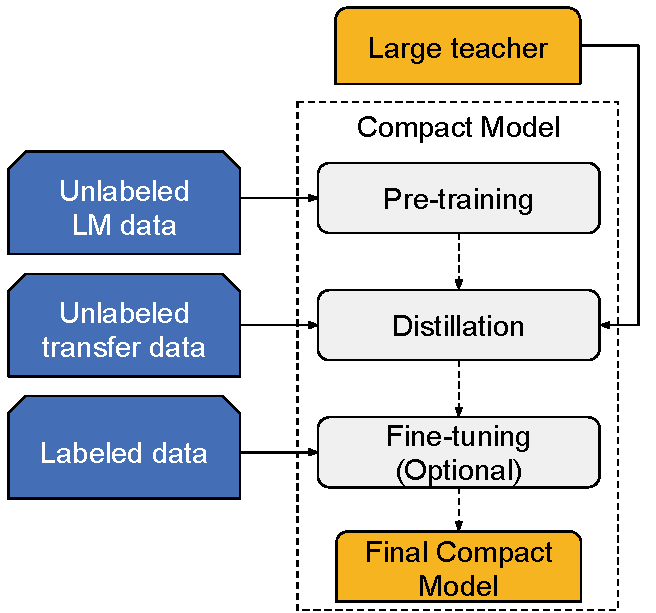
\includegraphics[width=\textwidth]{figures/recolored_our_recipe2.pdf}
        } % end scalebox
    \end{minipage}
    \caption{\recipename}
    \label{fig:pd}
\vspace{-10pt}
\end{figure}